%% Seminar deck for the X6CrNiNb18-10 point defect model identifiability study.
%%
%% Every number on these slides is quoted from a committed artefact under
%% outputs/paper/ (referee_stats.json, table1_parameters.csv,
%% table2_model_ladder.csv, table4_f1_exhibit.csv, table8_envelope_factors.csv,
%% table10_pbr_closure.csv).  Do not retype a value here from memory; see
%% docs/REPRODUCE.md for the command behind each one.
%%
%% Structure follows the talk brief: question, problem, gap, model, approach,
%% code, results, takeaway, limitations.
%%
%% Build:  latexmk -pdf slides.tex

\documentclass[aspectratio=169,10pt]{beamer}
\usetheme{metropolis}
\metroset{block=fill,numbering=fraction,progressbar=frametitle,sectionpage=progressbar}

\usepackage{amsmath,amssymb}
\usepackage{booktabs}
\usepackage{graphicx}
\usepackage{tikz}
\usetikzlibrary{arrows.meta,positioning,decorations.pathmorphing,patterns,fit,backgrounds,calc}

%% The deck keeps its own copies so talk/ is self-contained and can be
%% handed over or zipped on its own.  Refresh them with
%% scripts/make_talk_figs.py after regenerating the paper figures; that
%% script reads the \includegraphics names below, so the two cannot drift.
\graphicspath{{figures/}}

\definecolor{barrier}{RGB}{31,110,160}
\definecolor{outer}{RGB}{200,110,40}
\definecolor{alloyc}{RGB}{110,110,120}
\definecolor{nizone}{RGB}{60,150,90}
\definecolor{warn}{RGB}{180,40,40}

\newcommand{\Lbl}{L_{\mathrm{bl}}}
\newcommand{\Lol}{L_{\mathrm{ol}}}
\newcommand{\Abl}{A_{\mathrm{bl}}}
\newcommand{\Cbl}{C_{\mathrm{bl}}}
\newcommand{\Cx}{C_{x}}
\newcommand{\PBR}{\mathrm{PBR}_{\mathrm{eff}}}

\title{Sparse data limit what a mechanistic corrosion model can predict}
\subtitle{Identifiability of a point defect model for oxide growth on AISI~347}
\author{Conrard Giresse Tetsassi Feugmo}
\institute{Department of Chemistry, Department of Physics \& Astronomy\\University of Waterloo}
\date{}

\begin{document}

\maketitle

% ================================================================ question ===
\section{The question}

\begin{frame}{The question}
\begin{block}{}
\large
When we fit a mechanistic corrosion model to a handful of measurements and
extrapolate it across a service lifetime, \textbf{what have the data
actually determined?}
\end{block}

\vspace{1.0em}
Not: does the model fit. It does.

\vspace{0.4em}
But: would a very different parameter set have fitted just as well, and
predicted something else entirely?

\vspace{1.0em}
\small
A model that fits is not the same as a model that is \emph{identified}.
If the data cannot separate two parameter sets, the fit is honest and the
extrapolation is still meaningless.
\end{frame}

% ================================================================= problem ===
\section{The problem}

\begin{frame}{The problem}
Mechanistic corrosion models are routinely
\begin{itemize}
  \item written with four to six adjustable parameters,
  \item fitted to a handful of measurements,
  \item and then extrapolated across a service lifetime.
\end{itemize}

\vspace{0.6em}
\begin{alertblock}{What is almost never tested}
Whether the data determine those parameters at all.
\end{alertblock}

\vspace{0.8em}
The distinction is inert while the model is used inside its calibration
window, and decisive the moment it is used outside one, which is the only
reason to build a mechanistic model in the first place.
\end{frame}

% ===================================================================== gap ===
\section{The gap}

\begin{frame}{The gap in the literature}
Point defect model parameter estimation goes back four decades.

\vspace{0.7em}
\begin{columns}[T]
\begin{column}{0.48\textwidth}
\textbf{What is done}
\begin{itemize}\small
  \item PDM fitted to impedance spectra, or to depth profiles
  \item four to six parameters against three to six data points
  \item confidence intervals and correlations \emph{sometimes} reported
\end{itemize}
\end{column}
\begin{column}{0.48\textwidth}
\textbf{What is missing}
\begin{itemize}\small
  \item no profile-likelihood characterisation
  \item no bootstrap identifiability analysis
  \item no separation of prior leverage from data leverage
\end{itemize}
\end{column}
\end{columns}

\vspace{0.9em}
\begin{block}{}
To our knowledge this is the first formal identifiability
characterisation of a point defect model fit. The tools are mature in
systems biology and in battery modelling; they have not been brought
here.
\end{block}

\vspace{0.4em}
\scriptsize
And for AISI~347 in this environment, prior work stops at empirical
per-element power laws: no shared physical parameter set, no assessment
of how far the fits extrapolate.
\end{frame}

% ============================================================ system, data ===
\section{The system and the data}

\begin{frame}{The system}
\begin{columns}[T]
\begin{column}{0.46\textwidth}
\small
Nb-stabilised austenitic stainless steel\\
\textbf{X6CrNiNb18-10} (AISI~347)

\vspace{0.5em}
Simulated boiling-water-reactor hydrothermal water
\begin{itemize}\small
  \item $240\,^\circ$C, $7$~MPa
  \item $0.4$~ppm dissolved O$_2$
  \item exposures $72$, $168$, $480$~h
\end{itemize}

\vspace{0.5em}
A \textbf{duplex} oxide forms: a thin Cr-rich barrier layer that
controls the kinetics, and a thicker, far more variable Fe-rich
outer layer.
\end{column}

\begin{column}{0.52\textwidth}
\centering
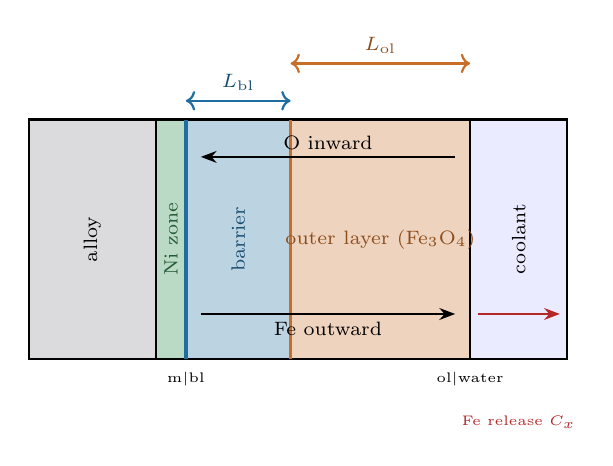
\begin{tikzpicture}[scale=0.95,every node/.style={font=\scriptsize}]
  \fill[alloyc!25] (0,0) rectangle (1.7,3.2);
  \fill[nizone!35]  (1.7,0) rectangle (2.1,3.2);
  \fill[barrier!30] (2.1,0) rectangle (3.5,3.2);
  \fill[outer!30]   (3.5,0) rectangle (5.9,3.2);
  \fill[blue!8]     (5.9,0) rectangle (7.2,3.2);

  \draw[thick] (0,0) rectangle (7.2,3.2);
  \draw[thick] (1.7,0)--(1.7,3.2);
  \draw[very thick,barrier] (2.1,0)--(2.1,3.2);
  \draw[very thick,outer] (3.5,0)--(3.5,3.2);
  \draw[thick] (5.9,0)--(5.9,3.2);

  \node[rotate=90] at (0.85,1.6) {alloy};
  \node[rotate=90,nizone!60!black] at (1.9,1.6) {Ni zone};
  \node[rotate=90,barrier!70!black] at (2.8,1.6) {barrier};
  \node[outer!70!black] at (4.7,1.6) {outer layer (Fe$_3$O$_4$)};
  \node[rotate=90] at (6.55,1.6) {coolant};

  \node[below] at (2.1,-0.05) {\tiny m$|$bl};
  \node[below] at (5.9,-0.05) {\tiny ol$|$water};

  \draw[<->,barrier,thick] (2.1,3.45)--(3.5,3.45) node[midway,above,barrier!70!black] {$\Lbl$};
  \draw[<->,outer,thick] (3.5,3.95)--(5.9,3.95) node[midway,above,outer!70!black] {$\Lol$};

  \draw[-{Stealth[length=2mm]},thick] (2.3,0.6)--(5.7,0.6) node[midway,below,yshift=1pt] {Fe outward};
  \draw[-{Stealth[length=2mm]},thick] (5.7,2.7)--(2.3,2.7) node[midway,above,yshift=-1pt] {O inward};
  \draw[-{Stealth[length=2mm]},thick,warn] (6.0,0.6)--(7.1,0.6);
  \node[warn,font=\tiny] at (6.55,-0.85) {Fe release $\Cx$};
\end{tikzpicture}

\vspace{0.2em}
{\tiny The barrier layer sets the kinetics; the outer layer is where the
information runs out.}
\end{column}
\end{columns}
\end{frame}

\begin{frame}{All of the calibration data}
\centering
\begin{tabular}{lrrr}
\toprule
$t$ (h) & Cr barrier (nm) & Fe outer (nm) & scans \\
\midrule
72  & $37.3 \pm 7.7$  & $143.3 \pm 111.5$ & 3 \\
168 & $98.3 \pm 21.7$ & $225.5 \pm 142.7$ & 4 \\
480 & $134.3 \pm 5.4$ & $240.3 \pm 172.5$ & 3 \\
\bottomrule
\end{tabular}

\vspace{1em}
\begin{columns}[T]
\begin{column}{0.48\textwidth}
\begin{alertblock}{Six numbers}
Three Cr, three Fe. Five fitted parameters.
\end{alertblock}
\end{column}
\begin{column}{0.48\textwidth}
\begin{alertblock}{Extrapolated 180-fold}
Last observation $480$~h $\rightarrow$ target $87\,600$~h.
\end{alertblock}
\end{column}
\end{columns}

\vspace{0.6em}
\small
The Fe standard deviations are $50$ to $70\%$ of the means. Whatever the
model says about the outer layer, the data barely constrain it.
\end{frame}

% =================================================================== model ===
\section{The model}

\begin{frame}{The reduced point defect model}
Barrier layer, from point defect kinetics with a field that relaxes as the
film thickens:
\[
  \frac{d\Lbl}{dt} \;=\; \Abl\, e^{\,b_3 \Lbl} \;-\; \Cbl ,
  \qquad \Lbl(0) = L_0 .
\]

Outer layer, fed by cations crossing the barrier and losing mass to the coolant:
\[
  \frac{d\Lol}{dt} \;=\; \PBR \, \frac{d\Lbl}{dt} \;+\; \Cx ,
  \qquad \Lol(0) = L_{\mathrm{ol},0} .
\]

\vspace{0.4em}
\begin{block}{One-way coupling, and why it matters}
$\Lbl$ never reads $\PBR$, $\Cx$ or $L_{\mathrm{ol},0}$. Every barrier-layer
result, including the ten-year prediction, is structurally immune to
everything the outer layer does. This is what lets us report an
outer-layer non-result without contaminating the headline number.
\end{block}

\vspace{0.3em}
\scriptsize
Reduced from a fourteen-reaction network; only four reactions displace a
boundary, and the constant-volume closure eliminates the cation fluxes.
\end{frame}

\begin{frame}{Closed form, and what we verify against it}
With $\Cbl = 0$ the barrier equation integrates exactly:
\[
  \Lbl(t) \;=\; L_0 - \frac{1}{b_3}\,
  \ln\!\Big( 1 - b_3\, \Abl\, e^{\,b_3 L_0}\, t \Big).
\]

\vspace{0.5em}
\begin{block}{Why this matters more than it looks}
A closed form means the inversion can be \textbf{graded against an exact
reference} rather than trusted. Most physics-informed inverse problems
have no such reference. This one does, and that is what makes the failure
mode later in this talk visible at all.
\end{block}

\vspace{0.5em}
\small
Closed form against stiff numerical integration: agreement to better than
$6\times10^{-11}$~nm. Any misfit we report is a statement about the data
and the model, never about the solver.
\end{frame}

% ================================================================ approach ===
\section{Our approach}

\begin{frame}{Our approach}
\centering
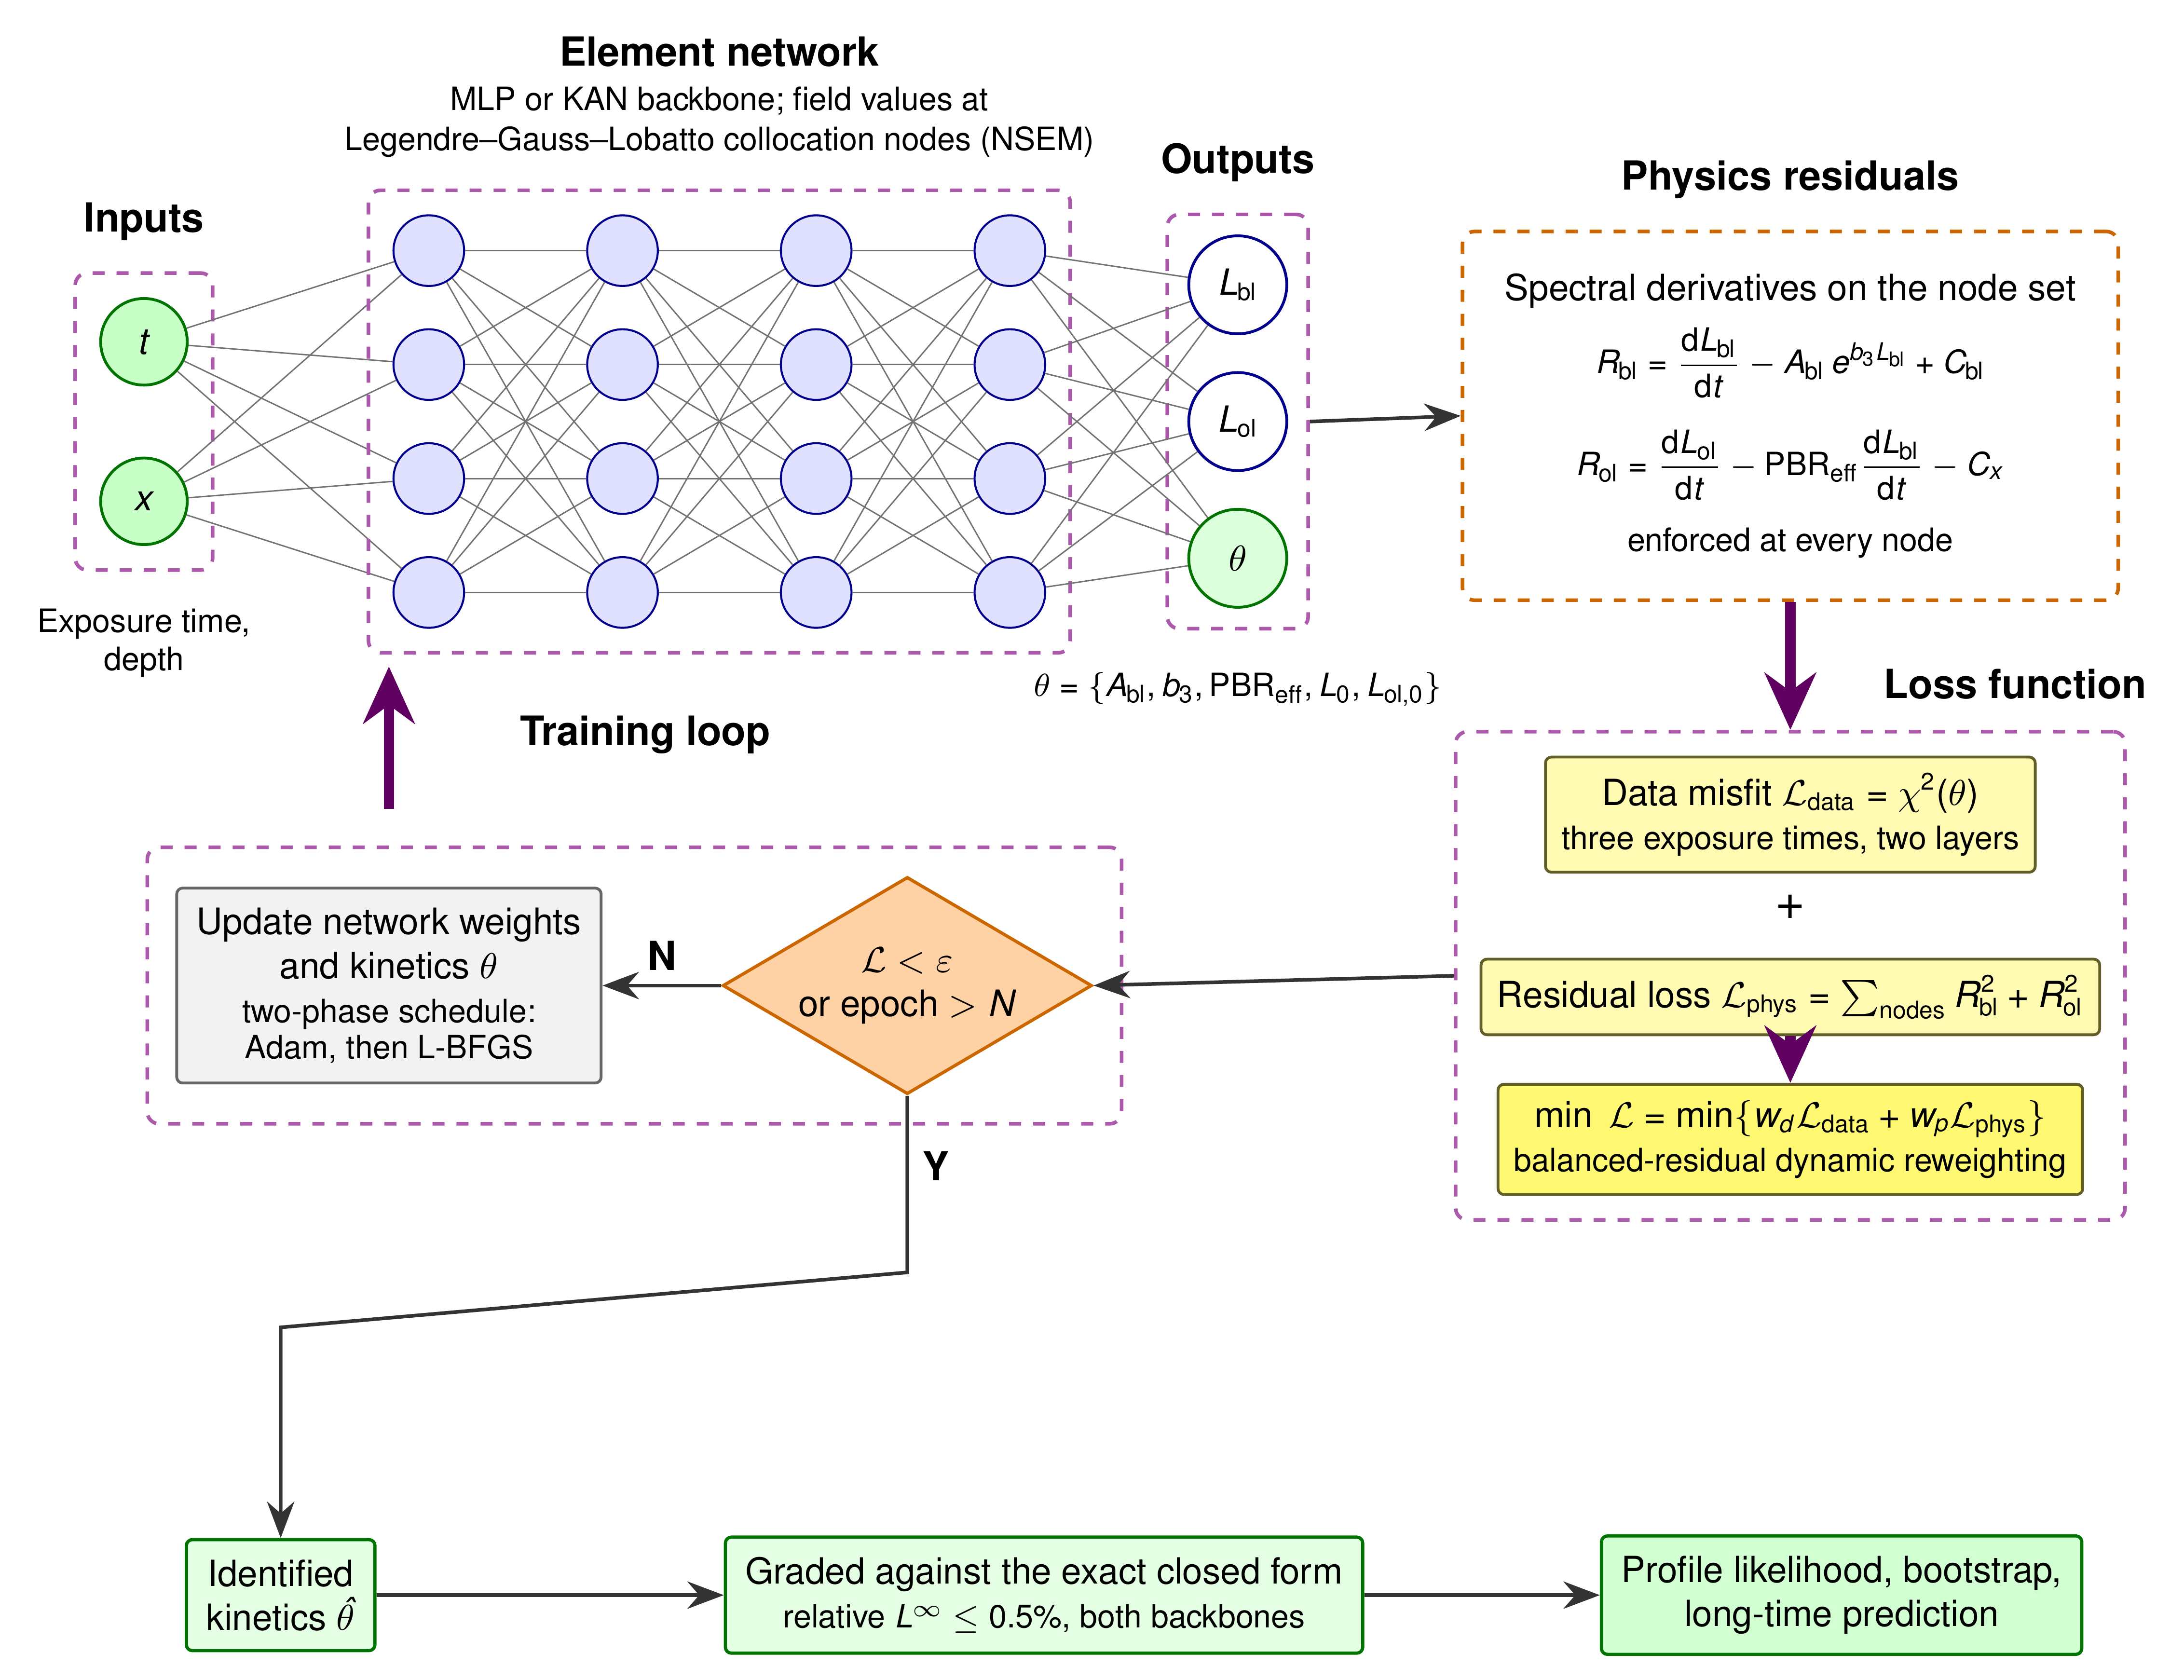
\includegraphics[height=0.66\textheight,keepaspectratio]{fig_nsem_workflow.png}

\vspace{0.4em}
\small
A \textbf{differentiable} inversion: exact parameter gradients through a
vectorised solver. Kinetics are recovered by hard-constrained inversion,
so the governing equations hold by construction, and checked against a
classical Levenberg--Marquardt fit.
\end{frame}

\begin{frame}{Identifiability, built in rather than bolted on}
Three tests, each capable of falsifying the fit:
\begin{enumerate}
  \item \textbf{Profile likelihood} across each parameter, with the others re-optimised.
  \item \textbf{Parametric bootstrap}, 1000 members, resampling at the measured scatter.
  \item \textbf{Prior relaxation}, to check a conclusion is not an artefact of a prior.
\end{enumerate}

\vspace{0.7em}
\begin{block}{What makes this affordable}
Differentiability, not the neural representation. Exact gradients are
what buy a thousand refits, sixty-one-point profile scans and a dense
operating-envelope grid. Closed-form models with automatic
differentiation share that property.
\end{block}

\vspace{0.5em}
\small And one comparison throughout: the same data fitted with a purely
empirical power law, then both extrapolated.
\end{frame}

% ==================================================================== code ===
\section{Our code}

\begin{frame}{Our code}
\begin{columns}[T]
\begin{column}{0.52\textwidth}
\textbf{An installable package}

\texttt{htw-pdm}, Apache~2.0\\
{\footnotesize\texttt{github.com/Feugmo-Group/x6crninb18-pdm}}

\vspace{0.6em}
\begin{itemize}\small
  \item classical fits, mass balance and spatial solves need only
        NumPy, SciPy, Matplotlib
  \item the neural inversions add the NSEM solver
  \item \textbf{71 tests} pin the reported numbers
\end{itemize}
\end{column}
\begin{column}{0.44\textwidth}
\textbf{A committed artefact per number}

\vspace{0.4em}
{\scriptsize
\begin{tabular}{ll}
\toprule
quantity & artefact \\
\midrule
parameters & \texttt{table1\_*.csv} \\
model ladder & \texttt{table2\_*.csv} \\
F-1 exhibit & \texttt{table4\_*.csv} \\
bootstrap, AIC & \texttt{referee\_stats.json} \\
\bottomrule
\end{tabular}}

\vspace{0.6em}
\small
A generated document maps every figure and table to the exact command
that produces it.
\end{column}
\end{columns}

\vspace{0.8em}
\begin{alertblock}{The rule we work to}
No number appears in the paper or on these slides unless a committed
artefact produces it. Retyping from memory is how the two drift.
\end{alertblock}
\end{frame}

% ================================================================= results ===
\section{Results}

\begin{frame}{Result 1: the model fits}
\begin{columns}[T]
\begin{column}{0.6\textwidth}
\centering
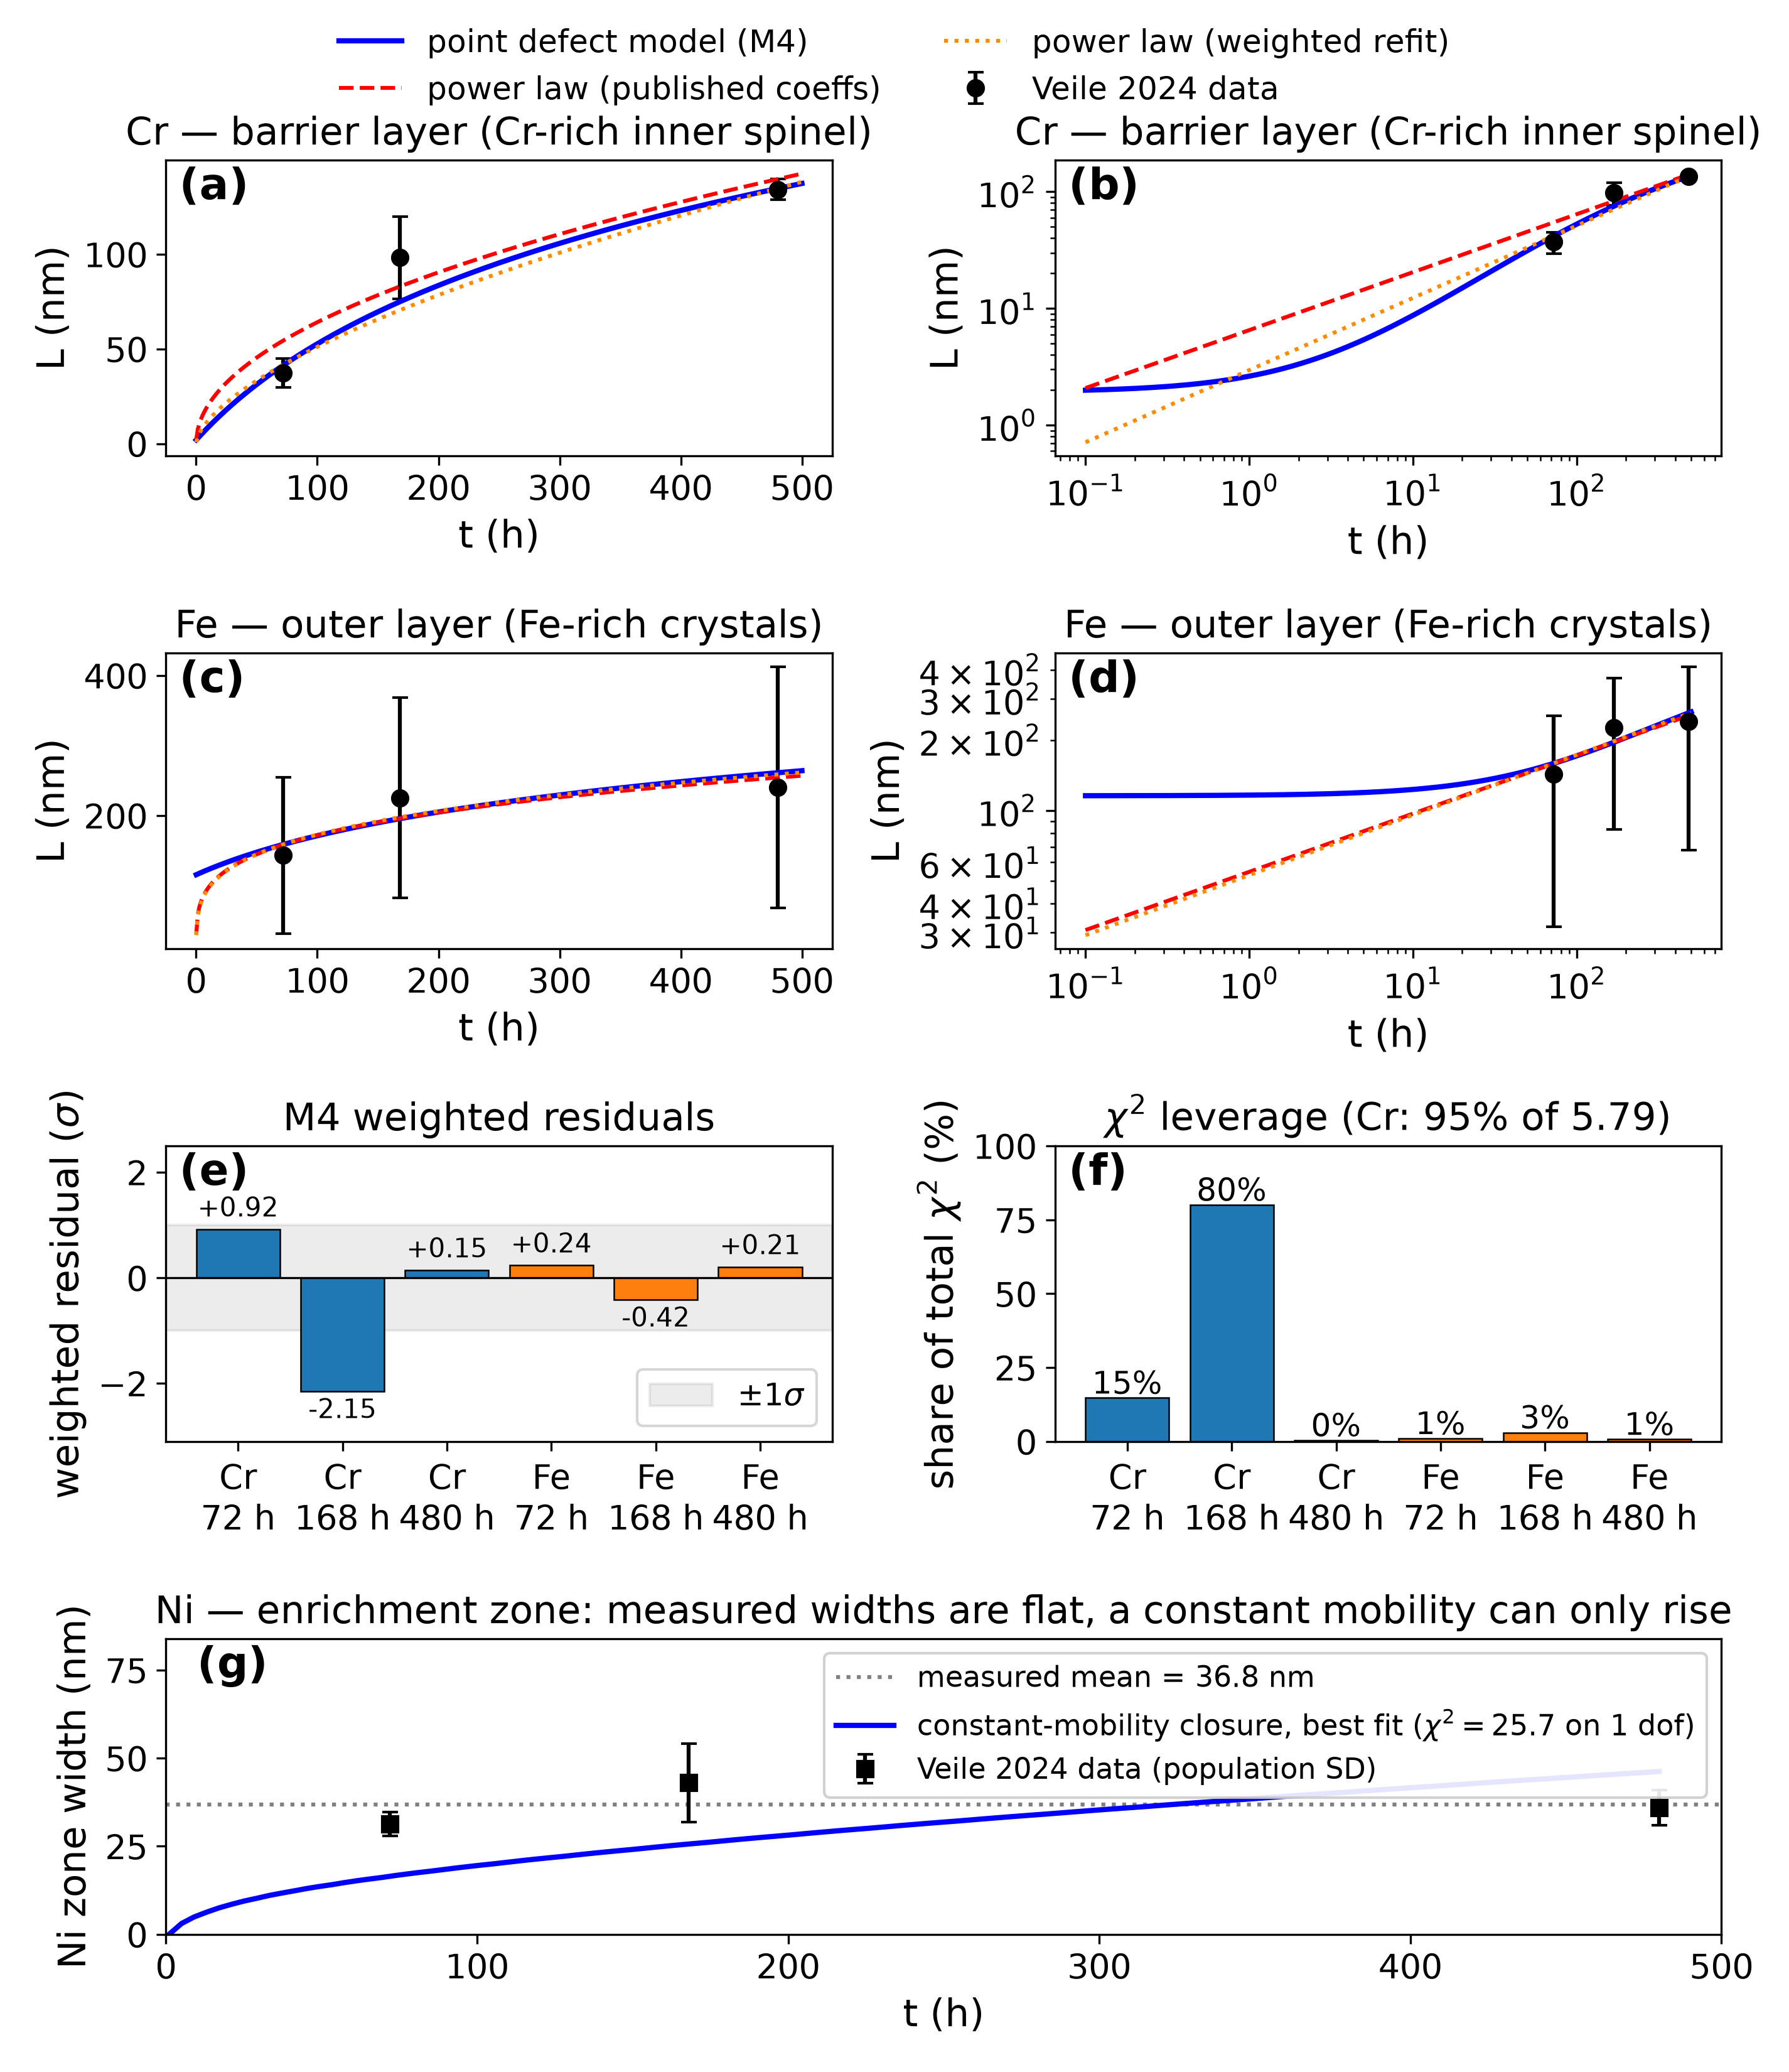
\includegraphics[width=\linewidth]{fig3_fits_vs_data.png}
\end{column}
\begin{column}{0.38\textwidth}
\small
Accepted model \textbf{M4}:
\[
\begin{aligned}
\Abl &= 0.7269~\mathrm{nm/h}\\
b_3 &= -0.012487~\mathrm{nm^{-1}}\\
\PBR &= 1.096\\
L_0 &= 1.924~\mathrm{nm}\\
L_{\mathrm{ol},0} &= 115.6~\mathrm{nm}
\end{aligned}
\]
\vspace{-0.3em}
\[\chi^2 = 5.79,\quad \mathrm{dof}=1\]

\vspace{0.4em}
{\footnotesize Refit under the same weighted objective, the empirical
power law reaches $\chi^2 = 7.84$ on $2$ dof. Comparable, not better.}
\end{column}
\end{columns}
\end{frame}

\begin{frame}{Result 2: but the fit is one measurement}
Weighted residual decomposition at M4:

\vspace{0.5em}
\centering
\begin{tabular}{lrrr}
\toprule
 & $72$~h & $168$~h & $480$~h \\
\midrule
Cr (barrier) & $+0.92$ & $\mathbf{-2.15}$ & $+0.15$ \\
Fe (outer)   & $+0.24$ & $-0.42$ & $+0.21$ \\
\bottomrule
\end{tabular}

\vspace{1em}
\begin{columns}
\begin{column}{0.48\textwidth}
\begin{alertblock}{95\%}
of $\chi^2$ sits on the three chromium points.
\end{alertblock}
\end{column}
\begin{column}{0.48\textwidth}
\begin{alertblock}{80\%}
sits on the single $168$~h chromium point.
\end{alertblock}
\end{column}
\end{columns}

\vspace{0.7em}
\small
The signs run $+$, $-$, $+$: a systematic curvature miss, not scatter.
And curvature is exactly what governs the extrapolation.
\end{frame}

\begin{frame}{Result 3: one parameter is not determined at all}
\begin{columns}[T]
\begin{column}{0.56\textwidth}
\centering
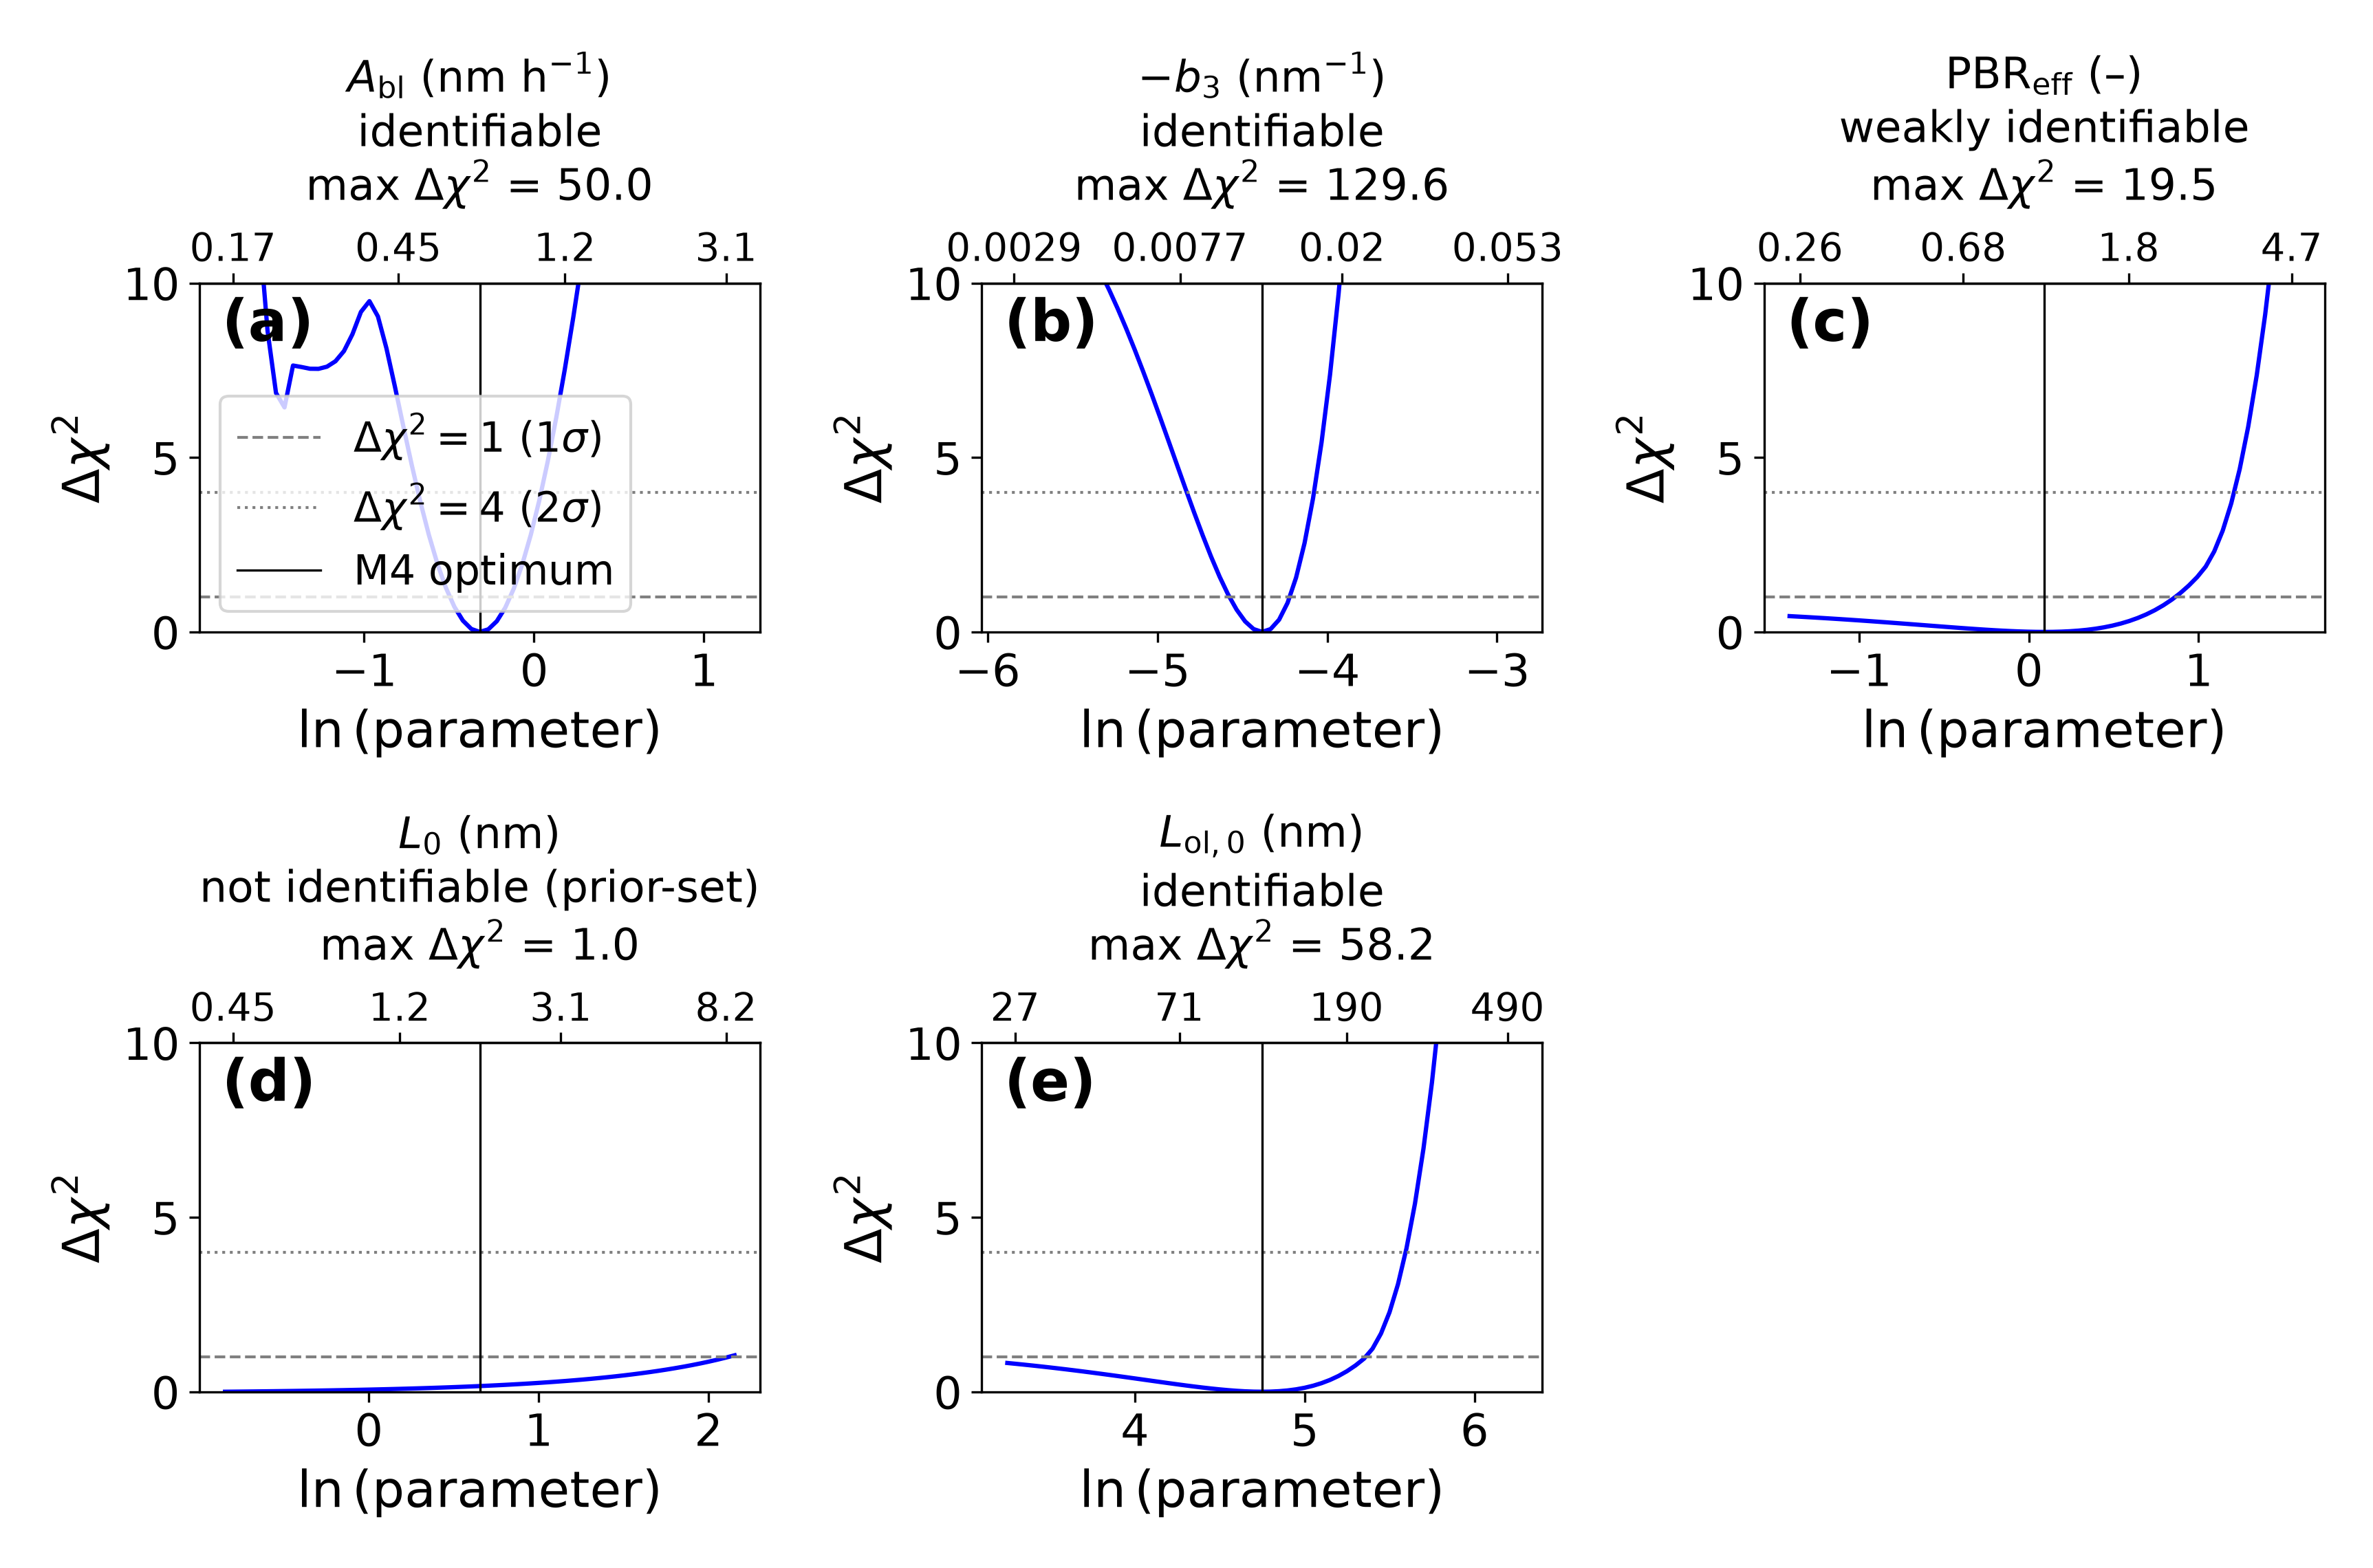
\includegraphics[width=\linewidth]{fig4_profile_likelihood.png}
\end{column}
\begin{column}{0.42\textwidth}
\scriptsize
\begin{tabular}{lrl}
\toprule
param & $\max\Delta\chi^2$ & verdict \\
\midrule
$b_3$   & $129.6$ & identifiable \\
$L_{\mathrm{ol},0}$ & $58.2$ & identifiable \\
$\Abl$  & $50.0$ & identifiable \\
$\PBR$  & $19.5$ & weakly id. \\
$L_0$   & $\mathbf{1.0}$ & \textcolor{warn}{unidentifiable} \\
\bottomrule
\end{tabular}

\vspace{0.8em}
\normalsize
$L_0$'s profile is \textbf{flat}: the data cannot move it. Its apparent
bootstrap precision ($1.92 \pm 0.04$~nm) is the prior speaking, not the
measurements.

\vspace{0.5em}
$\PBR$ spans $[0.25,\,2.32]$ at $1\sigma$.
\end{column}
\end{columns}
\end{frame}

\begin{frame}{Result 4: profile and bootstrap disagree, and that is the finding}
\centering

\includegraphics[height=0.60\textheight]{fig5_uncertainty_ensemble.png}

\vspace{0.4em}
\small
1000 members, zero failures. Two annotated features are results, not
plotting artefacts: the \textbf{spike at zero} for $\PBR$ and
$L_{\mathrm{ol},0}$ is what weak identifiability looks like under
resampling; the \textbf{narrow histogram} for $L_0$ is a prior, not a
constraint.
\end{frame}

\begin{frame}{Result 5: the key result}
\begin{columns}[T]
\begin{column}{0.54\textwidth}
\centering
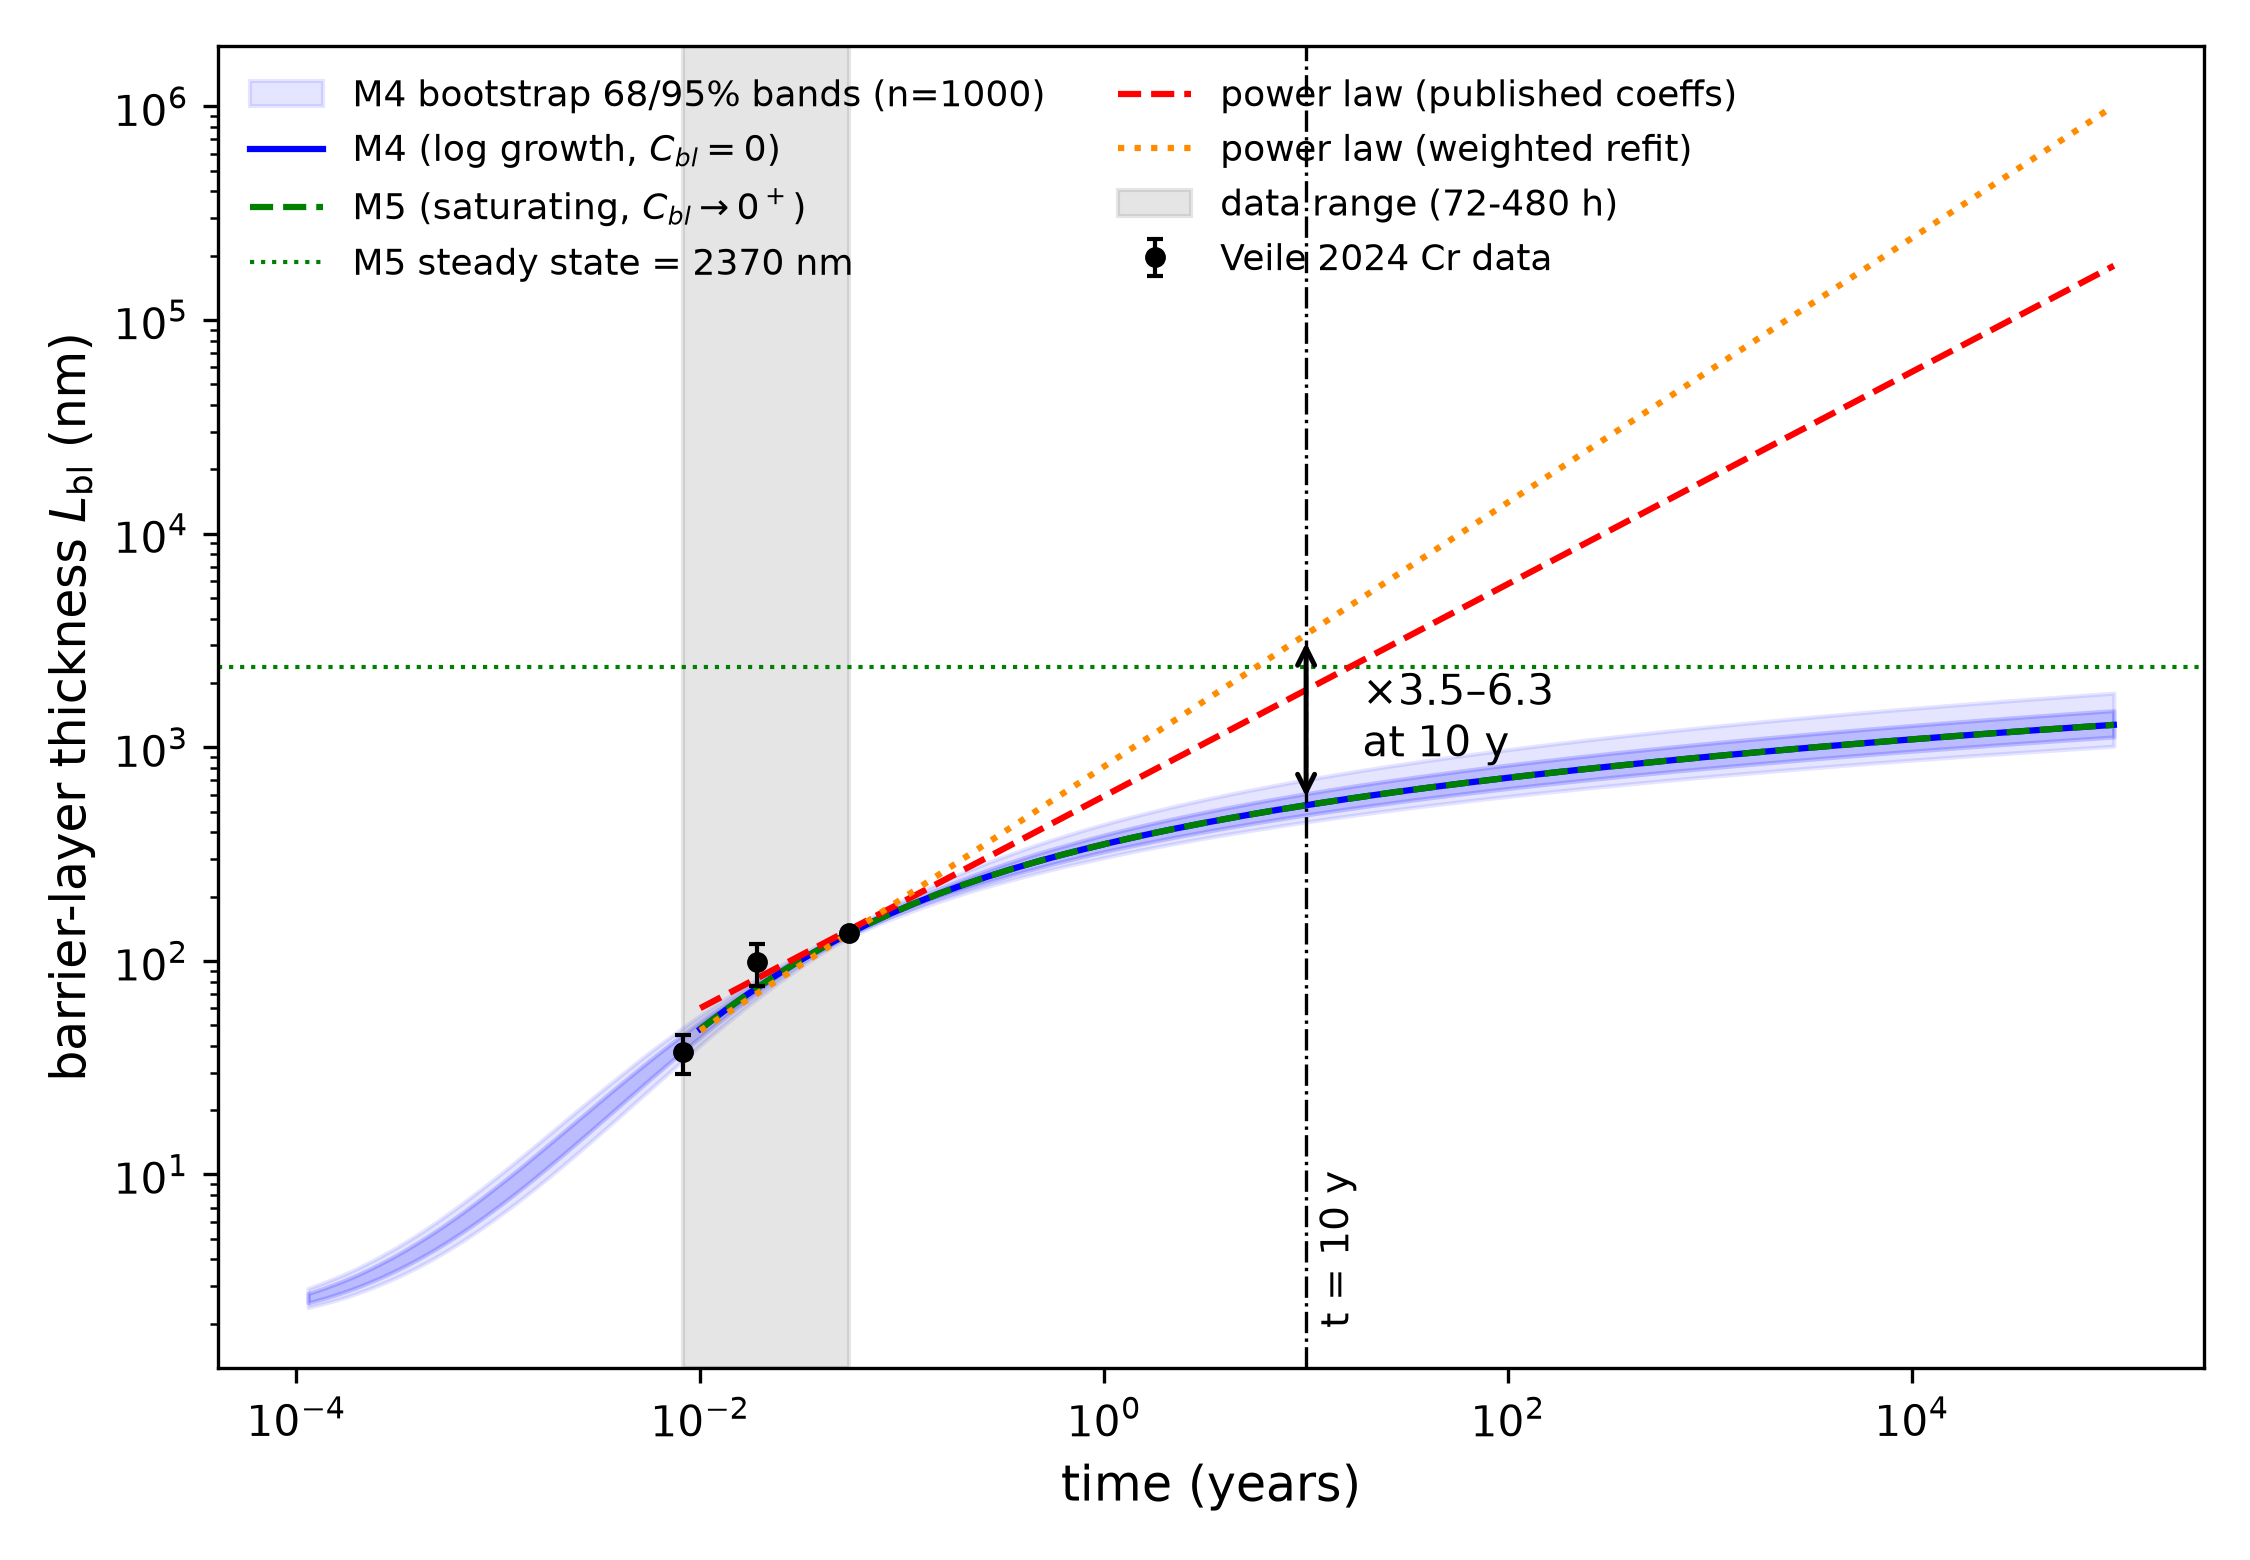
\includegraphics[width=\linewidth]{fig6_long_time.png}
\end{column}
\begin{column}{0.44\textwidth}
\begin{alertblock}{Same data, divergent futures}
Ten-year barrier thickness\\[2pt]
mechanistic \quad $535$~nm\\
power law \quad\; $1853$ to $3375$~nm\\[3pt]
a factor of \textbf{3.5 to 6.3}
\end{alertblock}

\vspace{0.6em}
\small
Bootstrap $95\%$ interval on the mechanistic value:
$[447,\,704]$~nm, widening to roughly $[340,\,1040]$~nm under the
maximal error rescaling.

\vspace{0.4em}
Both power-law variants lie outside that band under every error
treatment we apply.
\end{column}
\end{columns}

\vspace{0.4em}
\centering
\small
\textbf{What these data determine is the separation, not the number it brackets.}
\end{frame}

\begin{frame}{Why you cannot choose between them on the data}
\centering
\begin{tabular}{lrrr}
\toprule
 & $\chi^2$/dof & AIC & BIC \\
\midrule
M4 (mechanistic)       & $5.79/1$ & $15.79$ & $\mathbf{14.75}$ \\
power law (refit)      & $7.84/2$ & $15.84$ & $15.01$ \\
\bottomrule
\end{tabular}

\vspace{1.2em}
\raggedright
\begin{alertblock}{$\Delta\mathrm{AIC} = 0.05$}
On $n = 6$ points the two models are \textbf{statistically
indistinguishable}, and they disagree six-fold about the thing we
actually want to know.
\end{alertblock}

\vspace{0.6em}
\small
This is the whole argument in one line. Model selection on the
calibration window carries essentially no information about the
extrapolation.
\end{frame}

\begin{frame}{So: design the experiment that settles it}
Exposure needed before the two forms separate:

\vspace{0.7em}
\centering
\begin{tabular}{llrr}
\toprule
error budget & power law & $2\sigma$ & $3\sigma$ \\
\midrule
future scatter only & refit      & $1437$~h & $2020$~h \\
future scatter only & published  & $2546$~h & $4014$~h \\
\midrule
full budget         & refit      & $1928$~h & $5493$~h \\
full budget         & published  & $\mathbf{2988}$~h & $5129$~h \\
\bottomrule
\end{tabular}

\vspace{1.0em}
\raggedright
\begin{block}{Recommendation}
A single designed exposure of roughly $\mathbf{3000}$~h discriminates the
mechanistic and empirical kinetics at $2\sigma$ against the \emph{full}
error budget: future scatter, mechanistic parametric uncertainty and
power-law fit uncertainty together.
\end{block}

\vspace{0.3em}
\scriptsize
$3\sigma$ needs $5000$ to $6000$~h and, because the power law's own
uncertainty grows with its prediction, is available only inside a window
that closes near $34\,000$~h.
\end{frame}

\begin{frame}{Result 6: a failure mode the exact reference exposes}
\begin{columns}[T]
\begin{column}{0.58\textwidth}
\centering
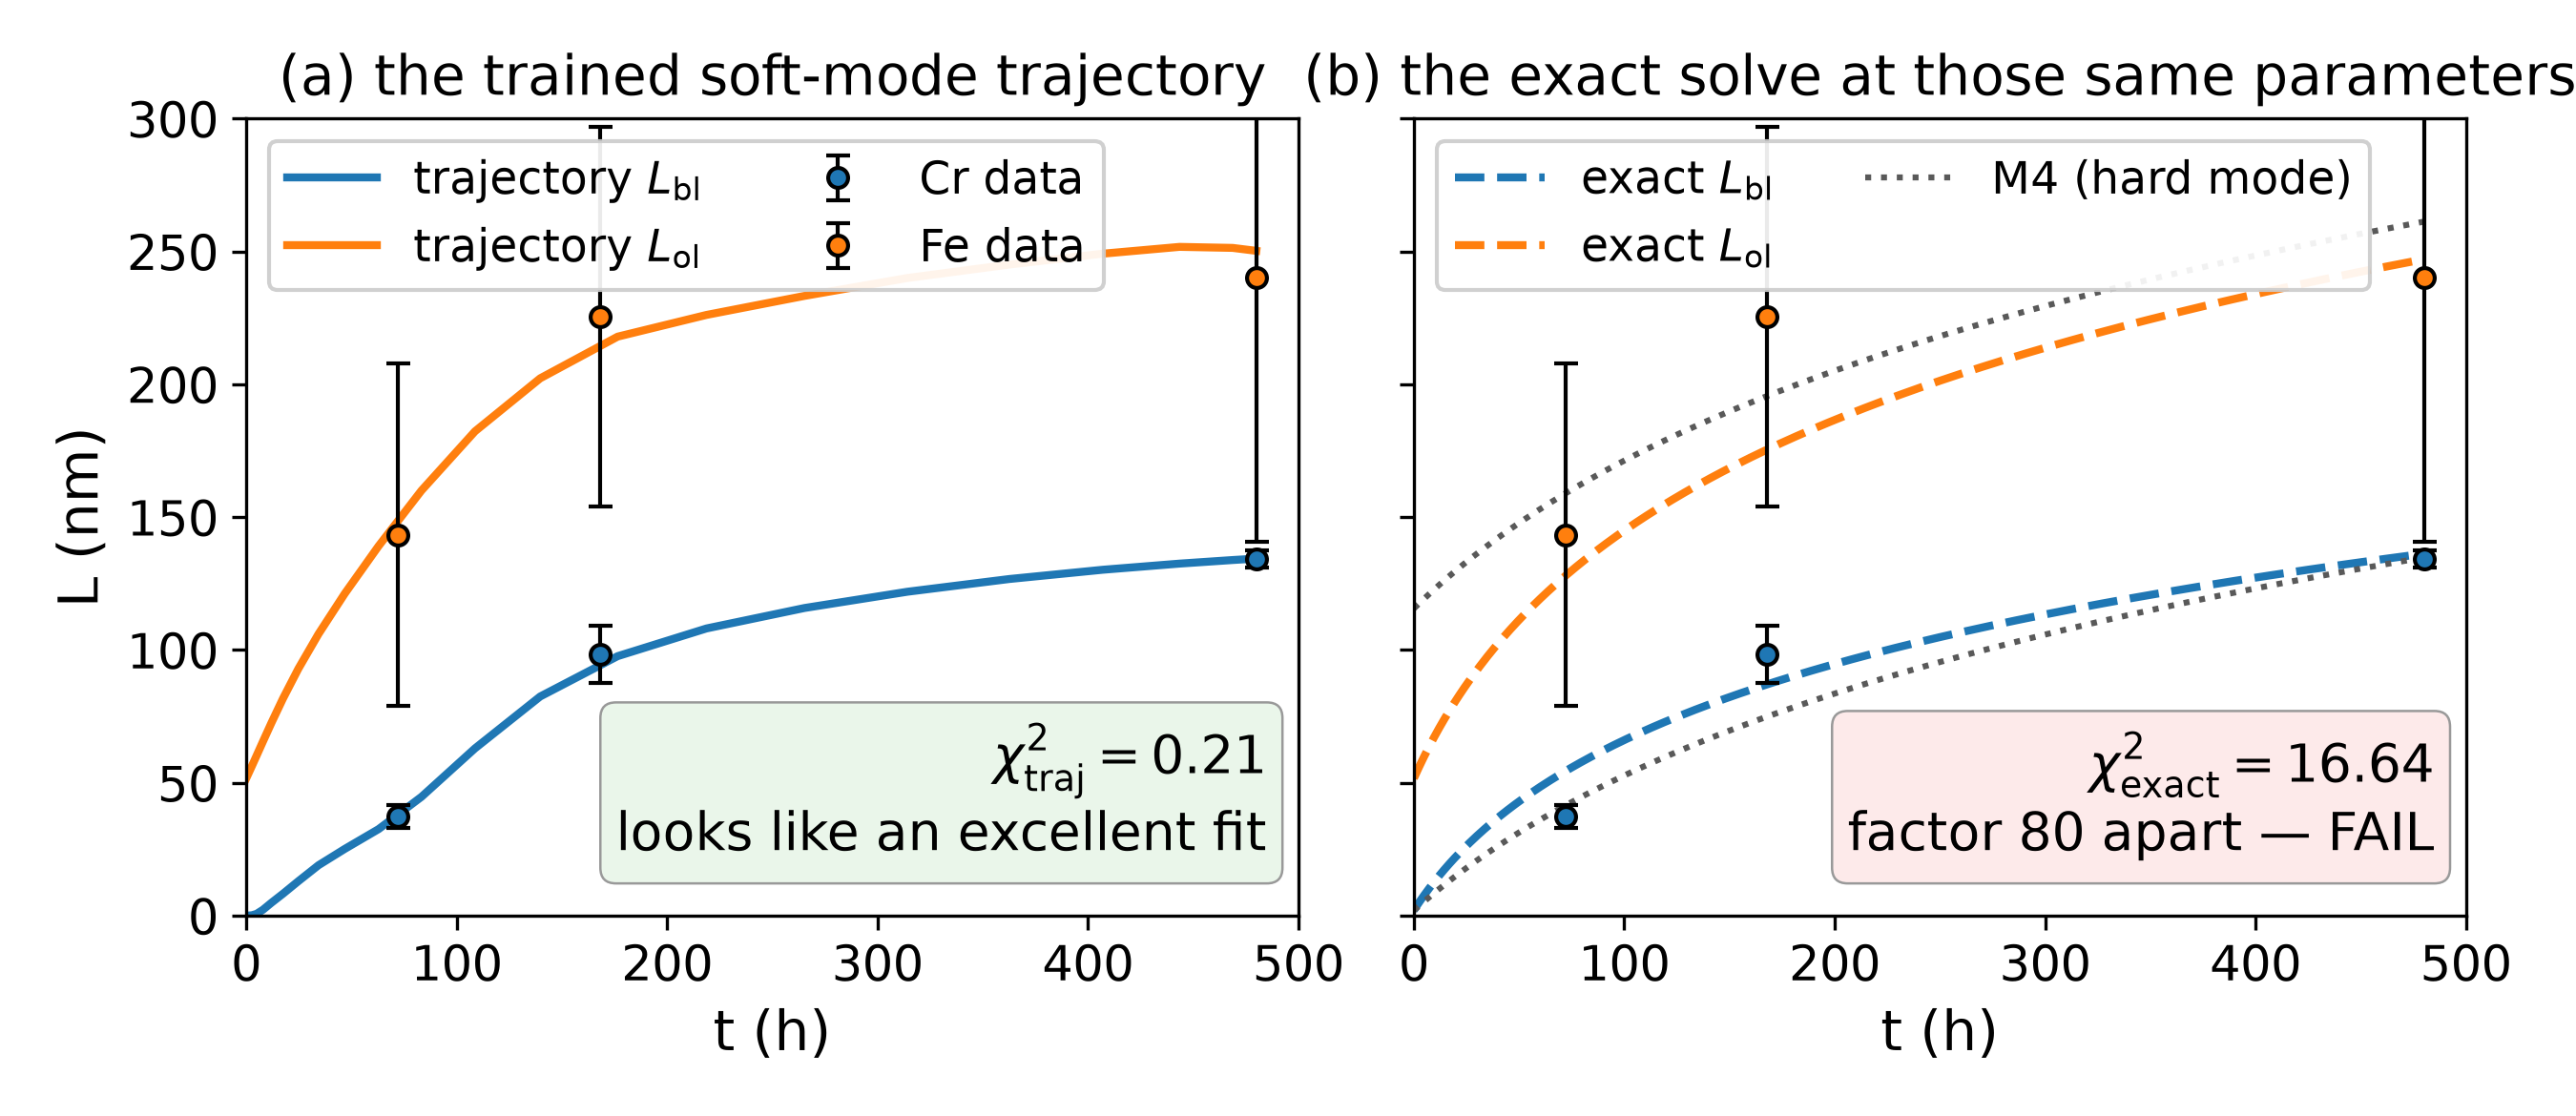
\includegraphics[width=\linewidth]{fig11_f1_failure.png}
\end{column}
\begin{column}{0.40\textwidth}
\small
Joint field-and-parameter training settles where the \textbf{data loss is
satisfied and the governing equation is not}.

\vspace{0.5em}
\centering
\scriptsize
\begin{tabular}{lrr}
\toprule
mode & $\chi^2_{\mathrm{traj}}$ & $\chi^2_{\mathrm{exact}}$ \\
\midrule
hard & $5.79$ & $5.79$ \\
soft, $\lambda_{\mathrm{phys}}$ & $0.21$ & $\mathbf{16.64}$ \\
soft, $\lambda_{\mathrm{data}}$ & $0.67$ & $\mathbf{15.57}$ \\
\bottomrule
\end{tabular}

\vspace{0.6em}
\raggedright
\normalsize
The trajectory \emph{looks} like a better fit than the accepted model.
The parameters it reports are wrong.
\end{column}
\end{columns}

\vspace{0.4em}
\small
\textbf{Remedy:} re-solve the recovered parameters through an independent
physics-exact forward solve and report that $\chi^2$ beside the training
one. We propose this alongside any physics-informed inverse result.
\end{frame}

\begin{frame}{Result 7: the spatial extension predicts composition for free}
\begin{columns}[T]
\begin{column}{0.48\textwidth}
\centering

\includegraphics[width=\linewidth]{fig10_composition_edx.png}
\end{column}
\begin{column}{0.48\textwidth}
\small
Extended spatially with \textbf{no additional free parameters}: every
kinetic parameter frozen at its zero-dimensional value.

\vspace{0.5em}
\begin{itemize}\small
  \item Cr plateau $46.7$ wt\% predicted against $\sim\!45$ measured
  \item layer widths matched to $+22\%$, $-20\%$, $+3\%$
\end{itemize}

\vspace{0.5em}
A structural argument, confirmed over four orders of magnitude in
diffusivity, shows quasi-steady composition data \textbf{cannot}
constrain the defect diffusivity however much is taken.
\end{column}
\end{columns}
\end{frame}

% ================================================================ takeaway ===
\section{Takeaway}

\begin{frame}{The takeaway}
\begin{enumerate}
  \item A reduced point defect model fits published depth-profile data for
        AISI~347 in BWR hydrothermal water, but \textbf{one of five
        parameters is undetermined} and a second only weakly determined.
  \item \textbf{95\% of the fit statistic rests on three points and 80\% on
        one}, with a systematic curvature miss. Single-number goodness of
        fit conceals this.
  \item Mechanistic and empirical kinetics are \textbf{indistinguishable on
        the calibration data} ($\Delta\mathrm{AIC} = 0.05$) yet differ
        \textbf{3.5 to 6.3 fold} at ten years.
  \item What the data determine is \textbf{the separation}, not the
        $535$~nm it brackets.
  \item \textbf{A designed exposure near $3000$~h would settle it.}
\end{enumerate}

\vspace{0.6em}
\begin{block}{The transferable point}
Report identifiability alongside goodness of fit, or the extrapolation is
not evidence. Nothing here is specific to this alloy or to the point
defect model.
\end{block}
\end{frame}

% ============================================================= limitations ===
\section{Limitations}

\begin{frame}{What this study cannot claim}
\begin{itemize}
  \item \textbf{Six data points.} No amount of further computation raises
        the information content. We add no new experiment.
  \item \textbf{The fit is formally rejected} at one degree of freedom:
        $\chi^2 = 5.79$ gives $p = 0.016$, and the error scale needed to
        make it acceptable is $s = 2.4$.
  \item \textbf{Part of the data is digitised} from a published figure.
  \item \textbf{The $[447, 704]$~nm interval understates the truth.} It is
        conditional on the model form, and the power-law comparison shows
        model-form uncertainty is roughly an order of magnitude larger.
  \item \textbf{One temperature, one oxygen level, unirradiated, static.}
        The operating-envelope map is a forward projection, not validation.
  \item \textbf{The neural solver was not needed.} Classical methods
        reproduce every result here, and in the spatial case more
        accurately. That is the point of a gradeable test case, not a
        defect of it.
\end{itemize}
\end{frame}

\begin{frame}[standout]
Questions
\end{frame}

% ================================================================== backup ===
\appendix

\begin{frame}{Backup: the model ladder}
\centering
\scriptsize
\begin{tabular}{lrrrrrr}
\toprule
model & extra & $n_{\mathrm{free}}$ & $\chi^2$ & $\Abl$ & $\PBR$ & $L_{\mathrm{ol},0}$ \\
\midrule
M1 core & --- & 4 & $7.15$ & $0.7516$ & $2.433$ & $0$ \\
M2 & $+\Cbl$ & 5 & $7.15$ & $0.7516$ & $2.433$ & $0$ \\
M3 & $+\Cbl+\Cx$ & 6 & $4.11$ & $955.8$ & $4.873$ & $0$ \\
\textbf{M4 (accepted)} & $+L_{\mathrm{ol},0}$ & 5 & $\mathbf{5.79}$ & $0.7269$ & $1.096$ & $115.6$ \\
M5 & $+L_{\mathrm{ol},0}+\Cbl$ & 6 & $5.79$ & $0.7269$ & $1.096$ & $115.6$ \\
power law (published) & $k,n$ per layer & 0 & $20.10$ & --- & --- & --- \\
power law (refit) & $k,n$ per layer & 4 & $7.84$ & --- & --- & --- \\
\bottomrule
\end{tabular}

\vspace{1em}
\raggedright
\small
M3 reaches a lower $\chi^2$ by running onto a degenerate ridge
($\Abl \approx \Cbl \approx 956$, $b_3 \to 0$), predicting $155$~nm at ten
years against M4's $535$. It is rejected on structure, not on fit. M5
recovers M4 exactly, confirming $\Cbl$ is redundant.
\end{frame}

\begin{frame}{Backup: the outer layer is exactly determined, so it says nothing}
\begin{columns}[T]
\begin{column}{0.5\textwidth}
\centering
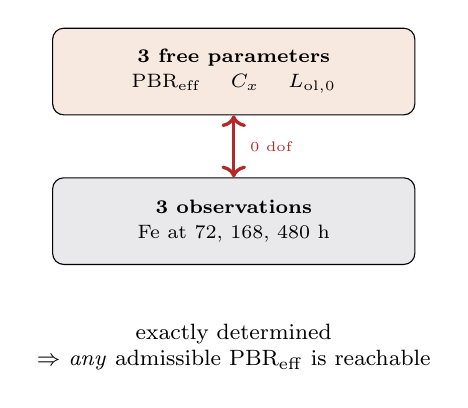
\begin{tikzpicture}[every node/.style={font=\scriptsize}]
  \node[draw,rounded corners,fill=outer!15,minimum width=46mm,minimum height=11mm,align=center] (p) at (0,1.6)
    {\textbf{3 free parameters}\\[1pt] $\PBR$ \quad $\Cx$ \quad $L_{\mathrm{ol},0}$};
  \node[draw,rounded corners,fill=alloyc!15,minimum width=46mm,minimum height=11mm,align=center] (d) at (0,-0.3)
    {\textbf{3 observations}\\[1pt] Fe at $72$, $168$, $480$~h};
  \draw[<->,very thick,warn] (p)--(d) node[midway,right,warn,font=\tiny,xshift=2pt] {0 dof};
  \node[align=center,font=\footnotesize] at (0,-1.9) {exactly determined\\$\Rightarrow$ \emph{any} admissible $\PBR$ is reachable};
\end{tikzpicture}
\end{column}
\begin{column}{0.48\textwidth}
\scriptsize
\begin{tabular}{lrr}
\toprule
$\PBR$ & $\Delta\chi^2$ & $\Cx$ (nm/h) \\
\midrule
$1.096$ (fit, $\Cx\!=\!0$) & --- & $0$ \\
$2.053$ (mass balance) & $-0.120$ & $-0.241$ \\
$2.156$ (with Ni routing) & $-0.131$ & $-0.264$ \\
$2.433$ (no precipitate) & $-0.157$ & $-0.327$ \\
\bottomrule
\end{tabular}

\vspace{0.8em}
\normalsize
The apparent factor-$1.9$ discrepancy between the fitted $\PBR$ and the
stoichiometric mass balance is \textbf{not a discrepancy}. The
stoichiometric value costs nothing; $\chi^2$ even improves.

\vspace{0.4em}
\footnotesize The data cannot separate iron \emph{production} from iron
\emph{loss to the coolant}.
\end{column}
\end{columns}
\end{frame}

\begin{frame}{Backup: a falsifiable by-product}
Imposing the stoichiometric ratio forces a specific outer-layer loss rate,
and therefore a specific iron release into the coolant:

\vspace{0.6em}
\centering
\begin{tabular}{lrr}
\toprule
$\PBR$ imposed & $\Cx$ (nm/h) & Fe release ($\mu$g\,dm$^{-2}$\,h$^{-1}$) \\
\midrule
$1.096$ & $-0.025$ & $0.94$ \\
$2.156$ & $-0.264$ & $\mathbf{9.94}$ \\
$2.433$ & $-0.327$ & $12.29$ \\
\bottomrule
\end{tabular}

\vspace{1em}
\raggedright
\small
A coolant-chemistry measurement discriminates these by an order of
magnitude. The non-result therefore comes with an experiment that would
convert it into a result.
\end{frame}

\begin{frame}{Backup: operating envelope}
\centering
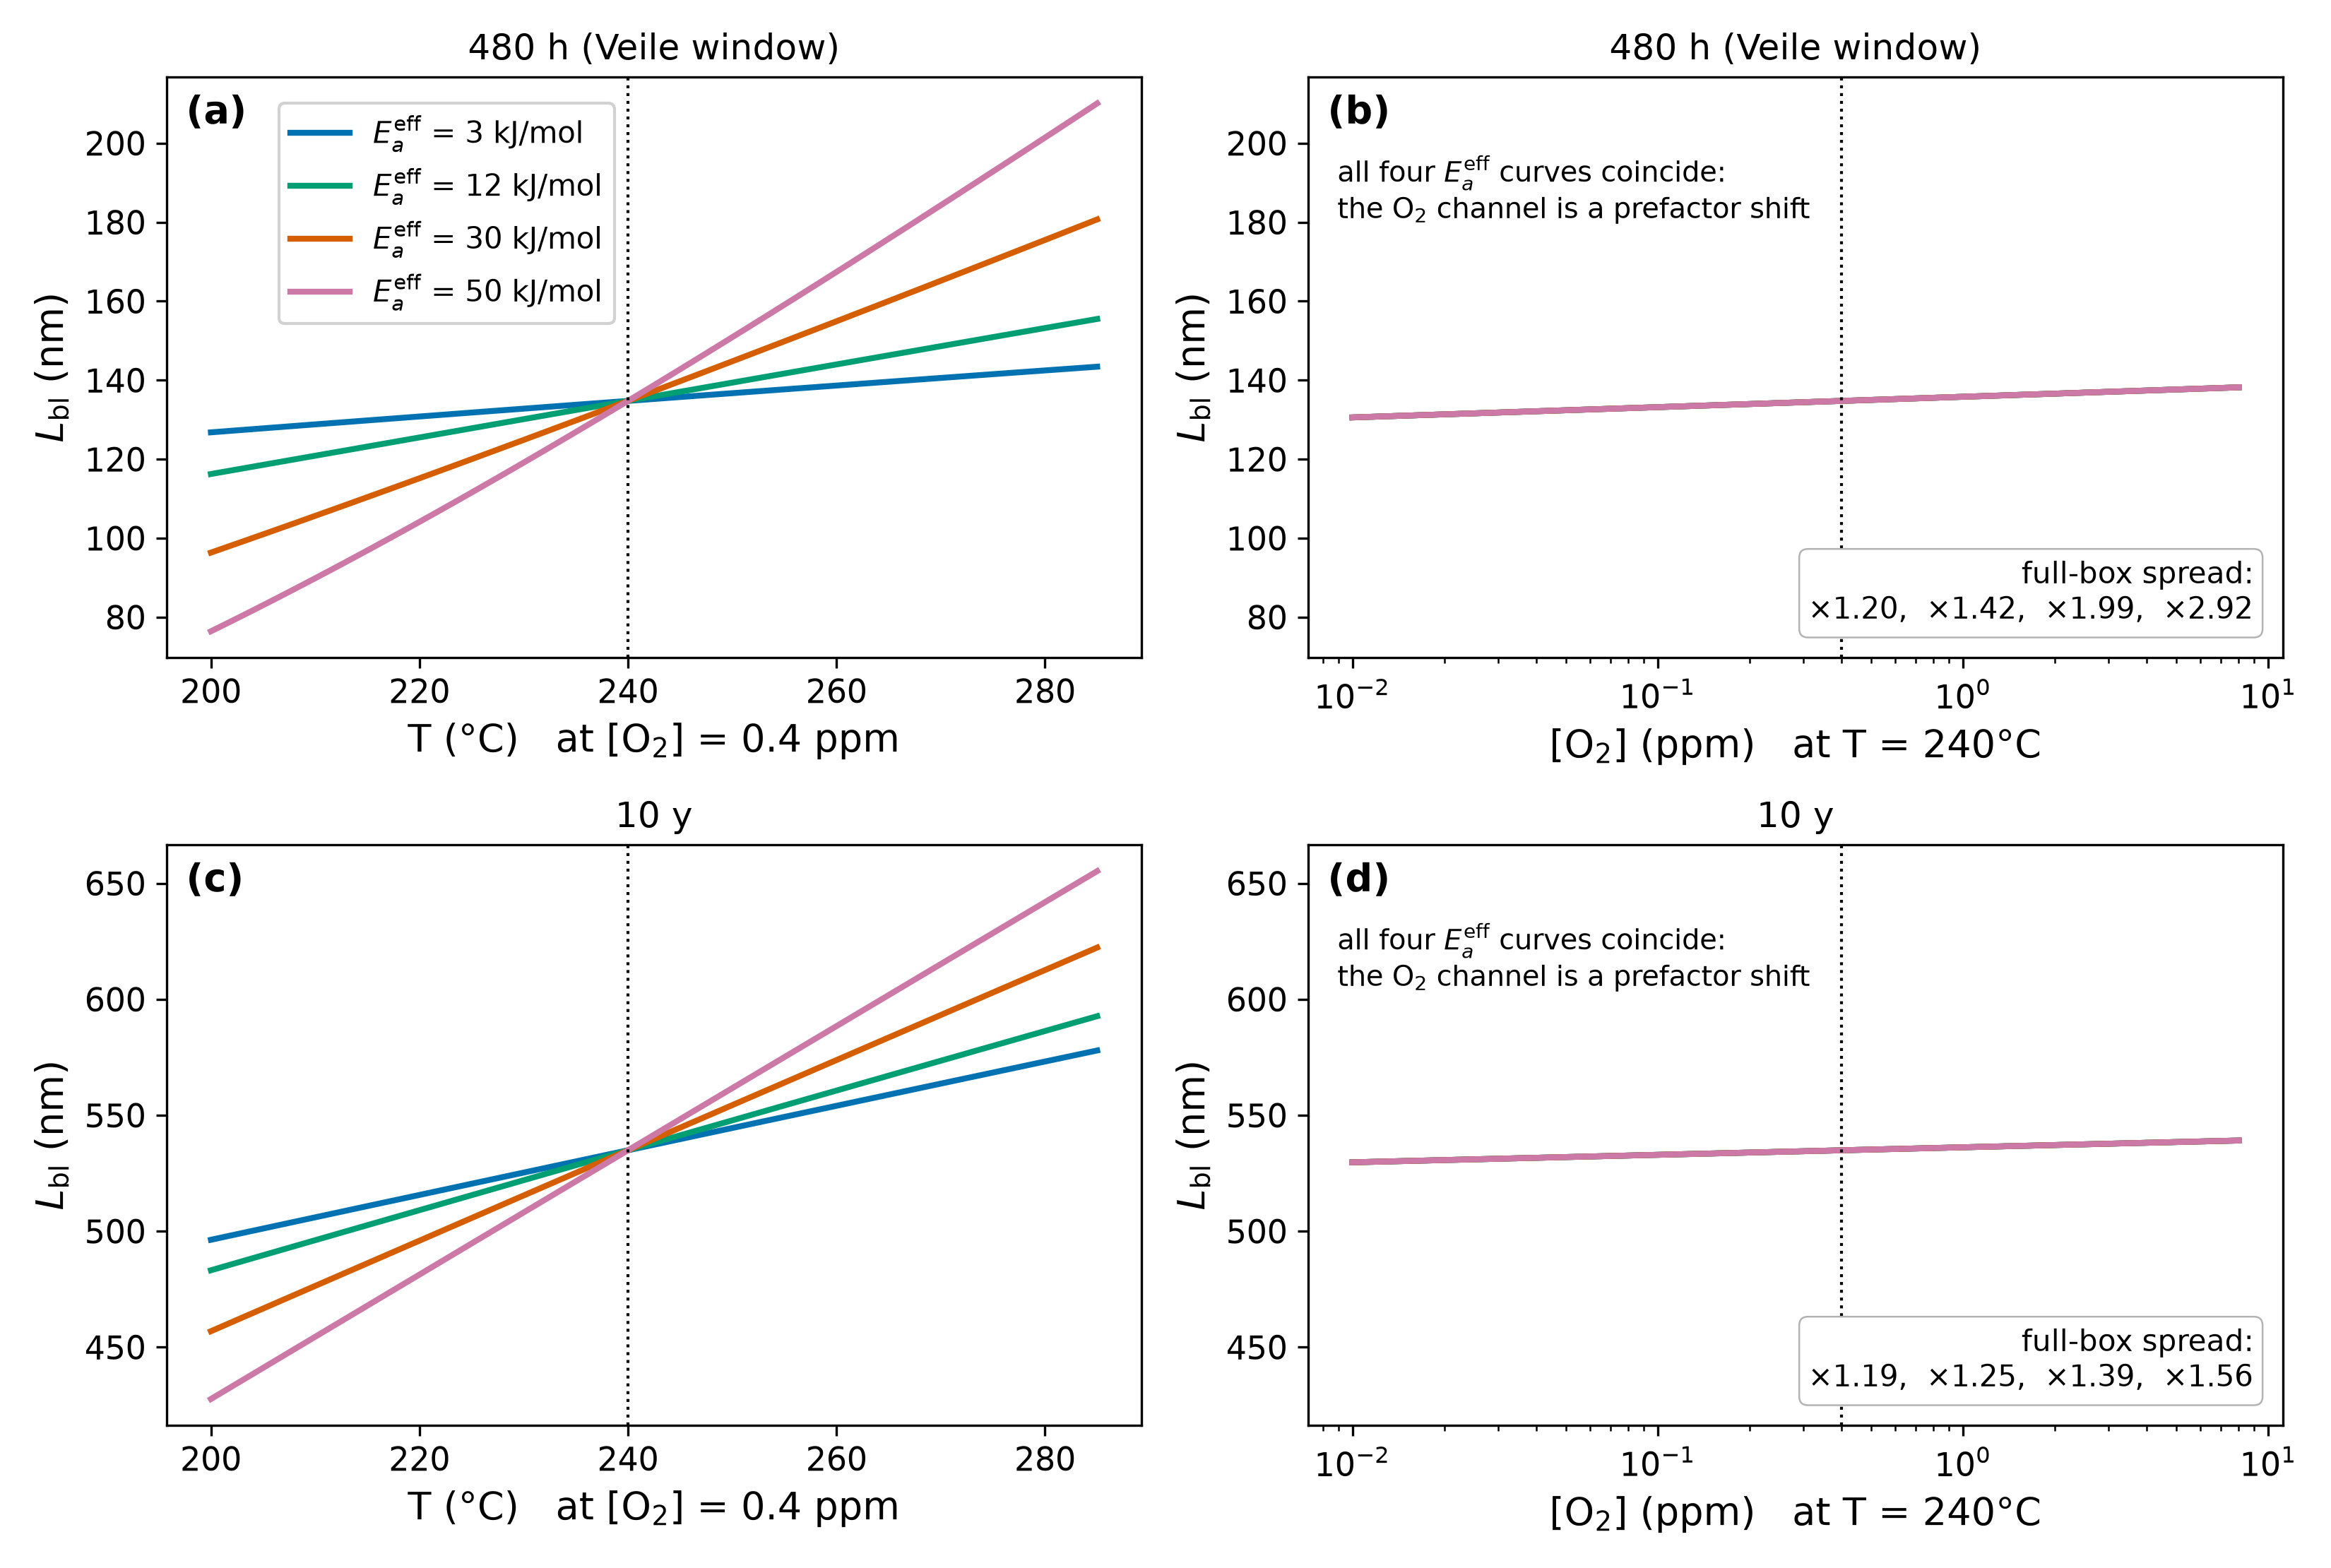
\includegraphics[height=0.62\textheight]{fig7_envelope_lines.png}

\vspace{0.3em}
\small
Across $200$--$285\,^\circ$C at $7$~MPa and $0.01$--$8$~ppm O$_2$, the
ten-year prediction varies by a factor of $1.19$ to $1.56$ depending on
the assumed activation energy. Small next to the $3.5$ to $6.3$ that the
choice of model form produces.
\end{frame}

\begin{frame}{Backup: does the constant-field closure hold?}
\centering
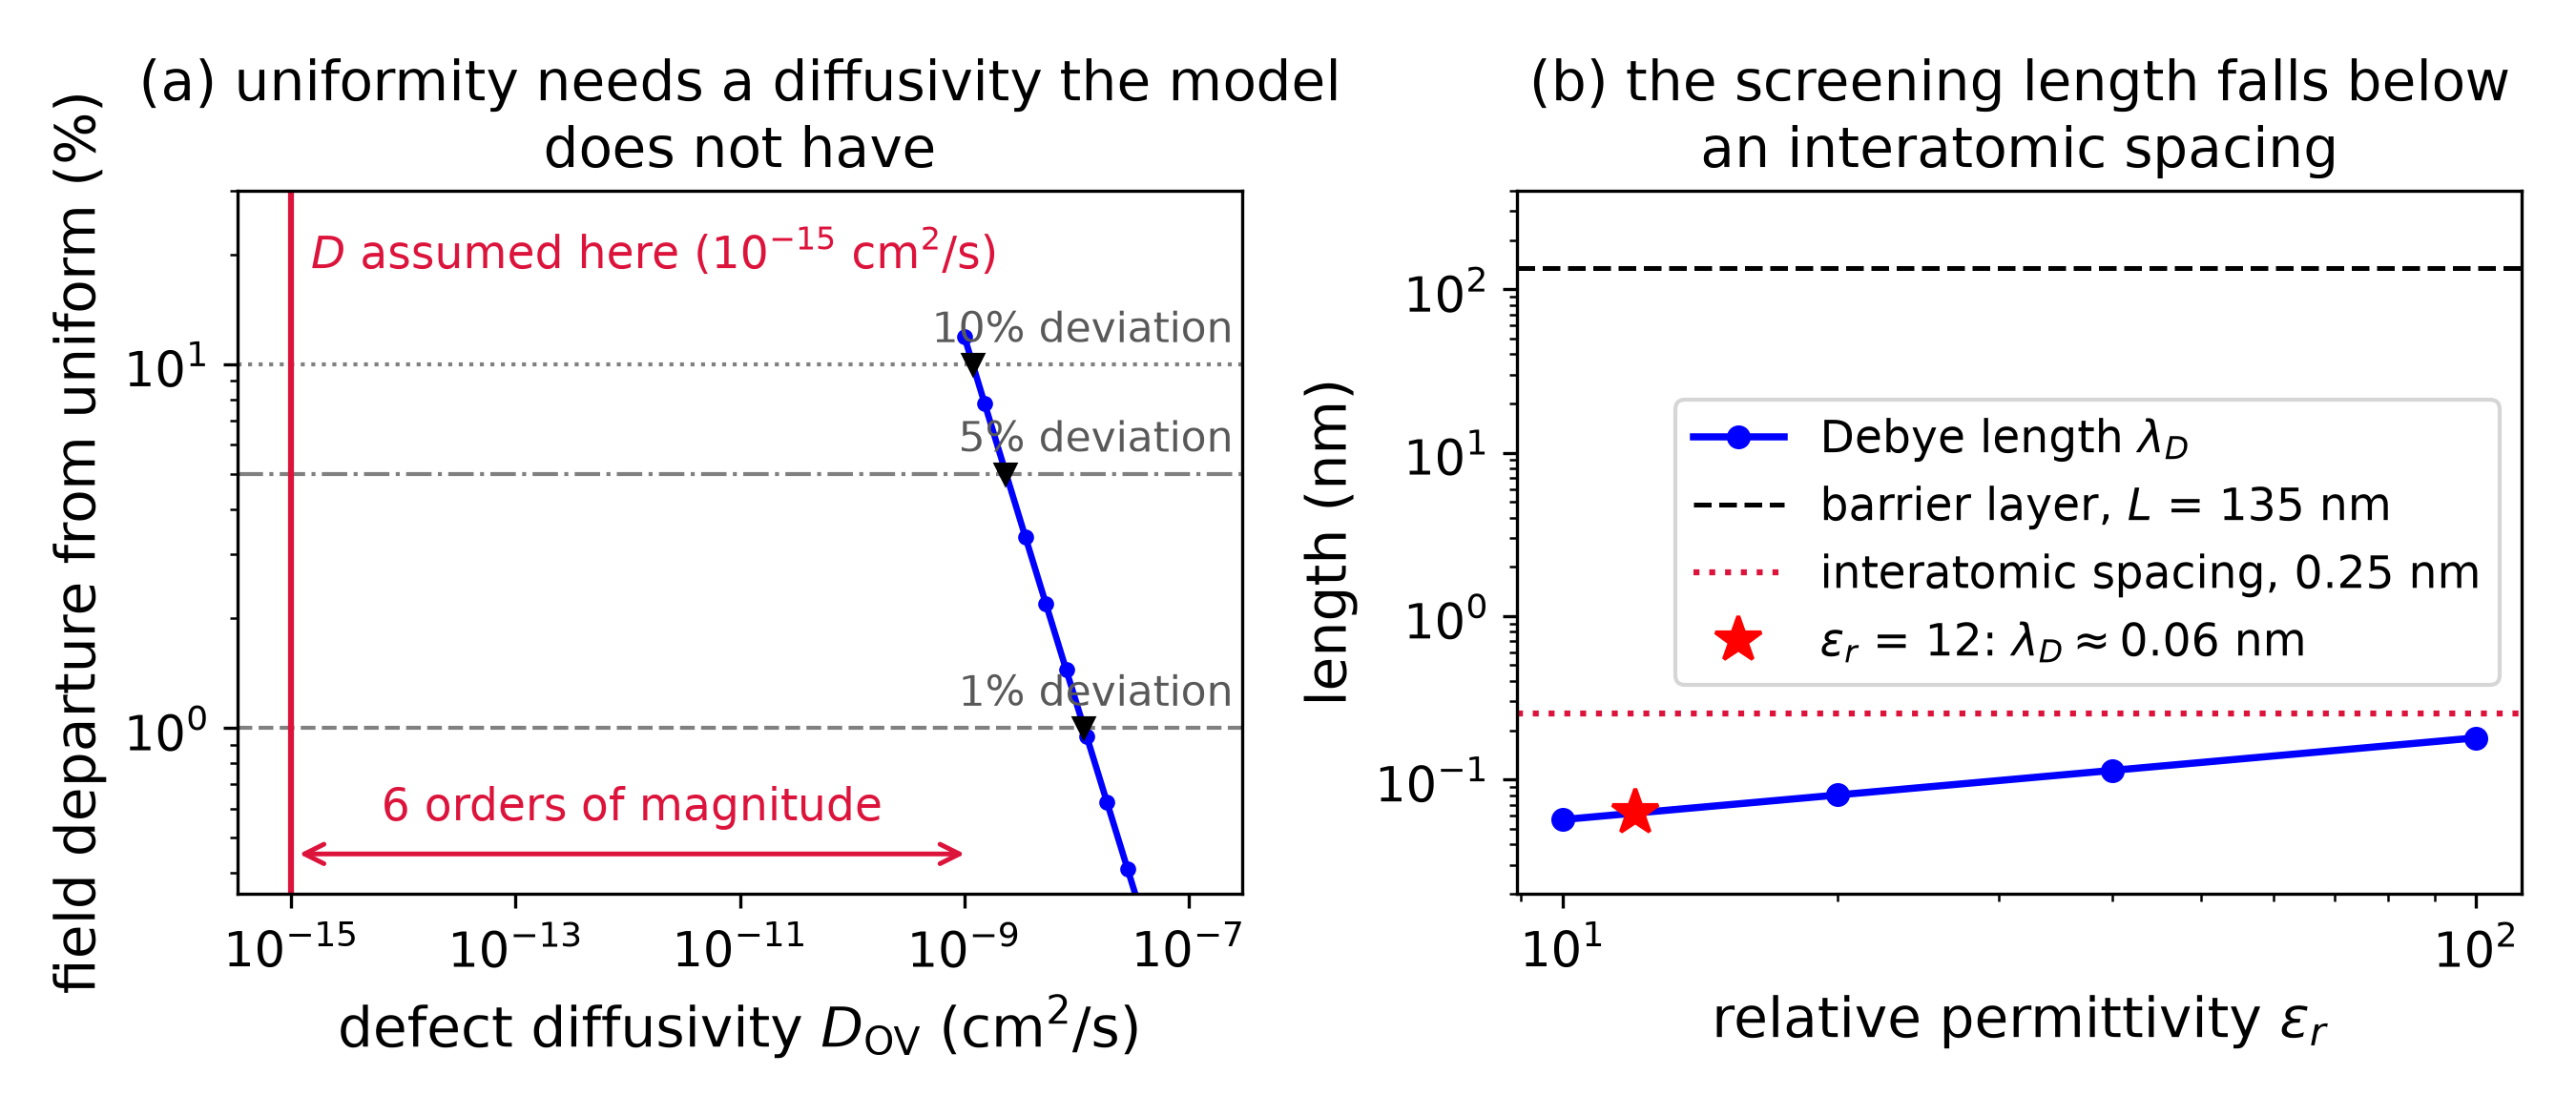
\includegraphics[height=0.60\textheight]{fig12_field_closure.png}

\vspace{0.3em}
\small
Solving Poisson's equation together with the defect transport, instead of
imposing the field, shows the PDM's constant-field closure is not
supported at the defect concentrations the model itself implies: the
implied Debye length is about $0.06$~nm, several times smaller than an
interatomic spacing. This leaves the fitted kinetics untouched, since the
identification is of $b_3$ and not of the field.
\end{frame}

\begin{frame}{Backup: reproducing every number}
\small
All quantities on these slides come from committed artefacts:

\vspace{0.6em}
\begin{tabular}{ll}
\toprule
slide content & artefact \\
\midrule
M4 parameters, profiles & \texttt{outputs/paper/table1\_parameters.csv} \\
model ladder & \texttt{outputs/paper/table2\_model\_ladder.csv} \\
F-1 exhibit & \texttt{outputs/paper/table4\_f1\_exhibit.csv} \\
envelope factors & \texttt{outputs/paper/table8\_envelope\_factors.csv} \\
bootstrap, AIC, power law & \texttt{outputs/paper/referee\_stats.json} \\
$\PBR$ closure, Fe release & \texttt{outputs/paper/table10\_pbr\_closure.csv} \\
\bottomrule
\end{tabular}

\vspace{1em}
The command behind each artefact is listed in
\texttt{docs/REPRODUCE.md}.
\end{frame}

\end{document}
